\documentclass[DaoFP]{subfiles}
\begin{document}
\setcounter{chapter}{15}

\chapter{Comonads}

If it were easily pronounceable, we should probably call side effects ``ntext,'' because the dual to side effects is ``context."

Just like we were using Kleisli arrows to deal with side effects, we use co-Kleisli arrows to deal with contexts. 

Let's start with the familiar example of an environment as a context. We have previously constructed a reader monad from it, by currying the arrow:
\begin{haskell}
(a, e) -> b
\end{haskell}
This time, however, we'll treat it as a co-Kleisli arrow, which is an arrow from a ``contextualized'' argument.

As was the case with monads, we are interested in being able to compose such arrows. This is relatively easy for the environment-carrying arrows:
\begin{haskell}
composeWithEnv :: ((b, e) -> c) -> ((a, e) -> b) -> ((a, e) -> c)
composeWithEnv g f = \(a, e) -> g (f (a, e), e)
\end{haskell}

It's also straightforward to implement an arrow that serves as an identity with respect to this composition:

\begin{haskell}
idWithEnv :: (a, e) -> a
idWithEnv (a, e) = a
\end{haskell}

This shows that there is a category in which co-Kleisli arrows serve as morphisms. 

\begin{exercise}
Show that the composition of co-Kleisli arrows using \hask{composeWithEnv} is associative.
\end{exercise}

\section{Comonads in Programming}

A functor \hask{w} (consider it a stylized upside-down \hask{m}) is a comonad if it supports composition of co-Kleisli arrows:

\begin{haskell}
class Functor w => Comonad w where
   (=<=) :: (w b -> c) -> (w a -> b) -> (w a -> c)
   extract :: w a -> a
\end{haskell}
Here, the composition is written in the form of an infix operator; and the unit of composition is called \hask{extract}, since it extracts a value from the context. 

Let's try it with our example. It is convenient to pass the environment as the first component of the pair. The comonad is then given by the functor that's a partial application of the pair constructor \hask{((,) e)}.
\begin{haskell}
instance Comonad ((,) e) where
  g =<= f = \ea -> g (fst ea, f ea)
  extract = snd
\end{haskell}

As with monads, co-Kleisli composition may be used in point-free style of programming. But we can also use the dual to \hask{join} called \hask{duplicate}:
\begin{haskell}
  duplicate :: w a -> w (w a)
\end{haskell}
or the dual to bind called \hask{extend}:
\begin{haskell}
  extend :: (w a -> b) -> w a -> w b
\end{haskell}
Here's how we can implement co-Kleisli composition in terms of \hask{duplicate} and \hask{fmap}:
\begin{haskell}
   g =<= f = g . fmap f . duplicate
\end{haskell}
\begin{exercise}
Implement \hask{duplicate} in terms of \hask{extend} and vice versa.
\end{exercise}
\subsection{The \hask{Stream} comonad}
Interesting examples of comonads deal with larger, sometimes infinite, contexts. Here's an infinite stream:
\begin{haskell}
data Stream a = Cons a (Stream a)
    deriving Functor
\end{haskell}

If we consider such a stream as a value of the type \hask{a} in the context of an infinite tail, we can provide a \hask{Comonad} instance for it:
\begin{haskell}
instance Comonad Stream where
  extract (Cons a as) = a
  duplicate (Cons a as) = Cons (Cons a as) (duplicate as)
\end{haskell}
Here, \hask{extract} returns the head of the stream and \hask{duplicate} turns a stream into a stream of streams, in which each consecutive stream is the tail of the previous one. 

The intuition is that \hask{duplicate} sets the stage for iteration, but it does it in a very general way. The head of each of the substreams can be interpreted as a possible ``current position'' in the original stream. 

It would be easy to perform a computation that goes over the head elements of these streams. But that's not where the power of a comonad lies. It lets us perform computations that require an arbitrary look-ahead.  Such a computation requires access not only to heads of consecutive substreams, but to their tails as well.

This is what \hask{extend} does: it applies a given co-Kleisli arrow to all the streams generated by \hask{duplicate}:
\begin{haskell}
  extend f (Cons a as) = Cons (f (Cons a as)) (extend f as)
\end{haskell}

Here's an example of a co-Kleisli arrow that averages the first five elements of a stream:
\begin{haskell}
avg :: Stream Double -> Double
avg  = (/5). sum . stmTake 5
\end{haskell}
It uses a helper function that extracts the first \hask{n} items:
\begin{haskell}
stmTake :: Int -> Stream a -> [a]
stmTake 0 _ = []
stmTake n (Cons a as) = a : stmTake (n - 1) as
\end{haskell}

We can run \hask{avg} over the whole stream using \hask{extend} to smooth local fluctuation. Electrical engineers might recognize this as a simple \index{low-pass filter}low-pass filter with \hask{extend} implementing the \index{convolution}convolution. It produces a running average of the original stream. 
\begin{haskell}
smooth :: Stream Double -> Stream Double
smooth = extend avg
\end{haskell}


Comonads are useful for structuring computations in spatially or temporally extended data structures. Such computations are local enough to define the ``current location,'' but require gathering information from neighboring locations. Signal processing or image processing are good examples. So are simulations, in which differential equations have to be iteratively solved inside volumes: climate simulations, cosmological models, or nuclear reactions, to name a few. Conway's Game of Life is also a good testing ground for comonadic methods.

Sometimes it's convenient to perform calculation on continuous streams of data, postponing the sampling until the very last step. Here's an example of a signal that is a function of time (represented by \hask{Double})
\begin{haskell}
data Signal a = Sig (Double -> a) Double
\end{haskell}
The first component is a continuous stream of \hask{a}'s implemented as a function of time. The second component is the current time.

This is the \hask{Comonad} instance for the continuous stream:
\begin{haskell}
instance Comonad Signal where
  extract (Sig f x) = f x
  duplicate (Sig f x) = Sig (\y -> Sig f (x - y)) x
  extend g (Sig f x) = Sig (\y -> g (Sig f (x - y))) x
\end{haskell}
Here, \hask{extend} convolves the filter 
\begin{haskell}
g :: Signal a -> a
\end{haskell}
over the whole stream. 

\begin{exercise}
Implement the \hask{Comonad} instance for a bidirectional stream:
\begin{haskell}
data BiStream a = BStr [a] [a]
\end{haskell}
Assume that both list are infinite. Hint: Consider the first list as the past (in reverse order); the head of the second list as the present, and its tail as the future.
\end{exercise}

\begin{exercise}
Implement a low-pass filter for \hask{BiStream} from the previous exercise, which averages over three values: the current one, one from the immediate past, and one from the immediate future. For electrical engineers: implement a Gaussian filter. 
\end{exercise}

\section{Comonads Categorically}

We can get the definition of a comonad by reversing the arrows in the definition of a monad. Our \hask{duplicate} corresponds to the reversed \hask{join}, and \hask{extract} is the reversed \hask{return}. 


A comonad is thus an endofunctor $W$ equipped with two natural transformations:
\begin{align*}
\delta &\colon W \to W \circ W \\
\varepsilon &\colon W \to \text{Id} 
\end{align*}

These transformations (corresponding to \hask{duplicate} and \hask{extract}, respectively) must satisfy the same identities as the monad, except with the arrows reversed. 

These are the counit laws:
\[
 \begin{tikzcd}
\text{Id} \circ W
 \arrow[rrd, "="']
& & W \circ W
 \arrow[ll, "\varepsilon \circ W"']
 \arrow[rr, "W \circ \varepsilon"]
&& W \circ \text{Id}
 \arrow[lld, "="]
 \\
 && W
  \arrow[u, "\delta"]
 \end{tikzcd}
\]
and this is the associativity law:
\[
 \begin{tikzcd}
 (W \circ W) \circ W 
 \arrow[rr, "="]
 &&
 W \circ (W \circ W)
 \\
 W \circ W 
 \arrow[u, "\delta \circ W"]
& & W \circ W
 \arrow[u, "W \circ \delta"']
 \\
&  W
 \arrow[ul, "\delta"]
 \arrow[ur, "\delta"']
 \end{tikzcd}
\]

\subsection{Comonoids}

We've seen how monadic laws followed from monoid laws. We can expect that comonad laws should follow from a dual version of a monoid. 

Indeed, a \index{comonoid}\emph{comonoid} is an object $w$ in a monoidal category $(\mathcal{C}, \otimes, I)$ equipped with two morphisms called co-multiplication and a co-unit:
\begin{align*}
\delta &\colon w \to w \otimes w \\
\varepsilon &\colon w \to I
\end{align*}
We can replace the tensor product with endofunctor composition and the unit object with the identity functor to get the definition of a comonad as a comonoid in the category of endofunctors.

In Haskell we can define a \hask{Comonoid} typeclass for the cartesian product:
\begin{haskell}
class Comonoid w where
  split   :: w -> (w, w)
  destroy :: w -> ()
\end{haskell}

Comonoids are less talked about than their siblings, monoids, mainly because they are taken for granted. In a cartesian category, every object can be made into a comonoid just by using the diagonal mapping $\Delta_a \colon a \to a \times a$ for co-multiplication, and the unique arrow to the terminal object for counit.

In programming this is something we do without thinking. Co-multiplication means being able to duplicate a value, and counit means being able to abandon a value. 

In Haskell, we can easily implement the \hask{Comonoid} instance for any type:
\begin{haskell}
instance Comonoid w where
  split w   = (w, w)
  destroy w = ()
\end{haskell}
In fact, we don't think twice of using the argument of a function twice, or not using it at all. But, if we wanted to be explicit, functions like:
\begin{haskell}
f x = x + x
g y = 42
\end{haskell}
could be written as:
\begin{haskell}
f x = let (x1, x2) = split x 
      in x1 + x1
g y = let () = destroy y 
      in 42
\end{haskell}

There are some situations, though, when duplicating or discarding a variable is undesirable. This is the case when the argument is an external resource, like a file handle, network port, or a chunk of memory allocated on the heap. Such resources are supposed to have well-defined lifetimes between being allocated and deallocated. Tracking lifetimes of objects that can be easily duplicated or discarded is very difficult and a notorious source of programming errors.

A programming model based on a cartesian category will always have this problem. The solution is to instead use a monoidal (closed) category that doesn't support duplication or destruction of objects. Such a category is a natural model for \index{linear types}\emph{linear types}.  Elements of linear types are used in \index{Rust}Rust and, at the time of this writing, are being tried in Haskell. In C++ there are constructs that mimic linearity, like \hask{unique_ptr} and move semantics.

\section{Comonads from Adjunctions}

We've seen that an adjunction $L \dashv R$ between two functors $L \colon \mathcal{D} \to \mathcal{C}$ and $R \colon \mathcal{C} \to \mathcal{D}$  gives rise to a monad $R \circ L \colon \mathcal{D} \to \mathcal{D}$. The other composition, $L \circ R$, which is an endofunctor in $\mathcal{C}$, turns out to be a comonad. 

The counit of the adjunction serves as the counit of the comonad. This can be illustrated by the following string diagram:
\[
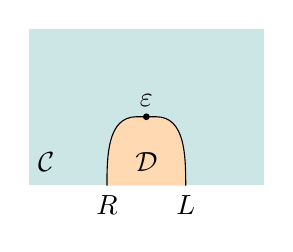
\begin{tikzpicture}
\def\xleft{0.5};
\def\xmid{1};
\def\xright{1.5};

\def \ybot{0};
\def \ymid{1};
\def \ytop{2 * \ymid};
%\def \yt{2 * \ymid - 0.3};
\def \yb{2 * \ybot + 0.3};

\node [below] (a) at (\xleft, \ybot) {$R$};
\node(b) [below] at (\xmid, \ymid) {};
\node[below] (c) at (\xright, \ybot) {$L$};

\filldraw[fill=blue!50!green!20, draw=white] (\xleft-1, \ytop) rectangle (\xright+1, \ybot);

\draw [fill=orange!30] (a.north) to [out=90, in=180] (b.west) -- (b.east) to [out=0, in=90] (c.north);

\filldraw[black] (b) circle (1 pt);
\node [above] at (b) {$\varepsilon$};

\node(l)[right] at (\xleft-1, \yb) {$\mathcal{C}$};
\node(r) at (\xmid, \yb) {$\mathcal{D}$};

\end{tikzpicture}
\]

The comultiplication is given by the whiskering of $\eta$:
\[ \delta = L  \circ \eta \circ R \]
as illustrated by this string diagram:
\[
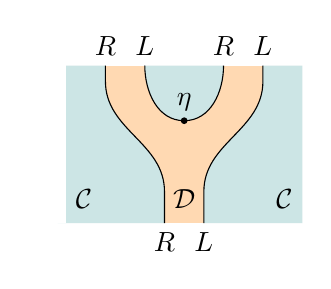
\begin{tikzpicture}
\def \xmid          {0};
\def \xr               {0.5};
\def \xrr             {1}
\def \xrm            {0.25}
\def \xrightmost {1.5}
\def \xl {-\xr}
\def \xll {-\xrr}
\def \xlm {-\xrm}
\def \xleftmost {-\xrightmost}

\def \ybot           {0};
\def \ymidbot     {-0.20};
\def \yeps          {-0.7};
\def \ymid          {-1};
\def \ymidtop     {-1.60}
\def \ytop           {-2};
\def \ylabel        {\ytop + 0.3};
% functors
\node [below] at (\xlm, \ytop)  {$R$};
\node [below] at (\xrm, \ytop) {$L$};

\node [above] at (\xll, \ybot) {$R$};
\node [above] at (\xl, \ybot) {$L$};
\node [above] at (\xr, \ybot) {$R$};
\node [above] at (\xrr, \ybot) {$L$};

\filldraw[fill=orange!30, draw=white] (\xleftmost, \ytop) rectangle (\xrightmost, \ybot);

% left area
\path [fill=blue!50!green!20] (\xleftmost, \ybot) to  (\xll, \ybot) to (\xll, \ymidbot) [out=-90, in=90] to (\xlm, \ymidtop) to  (\xlm, \ytop) to [out=180, in=180] (\xleftmost, \ytop);
% right area
\path [fill=blue!50!green!20] (\xrightmost, \ybot) to (\xrr, \ybot) to (\xrr, \ymidbot) [out=-90, in=90] to (\xrm, \ymidtop) to (\xrm, \ytop) to [out=0, in=180]  (\xrightmost, \ytop);
% cap
\draw [fill=blue!50!green!20] (\xl, \ybot) to [out=-90, in=180] (\xmid, \yeps) to [out=0, in=-90] (\xr, \ybot);
% left curve
\draw (\xll, \ybot) to (\xll, \ymidbot) [out=-90, in=90] to (\xlm, \ymidtop) to  (\xlm, \ytop);
% right curve
\draw (\xrr, \ybot) to (\xrr, \ymidbot) [out=-90, in=90] to (\xrm, \ymidtop) to (\xrm, \ytop);
% eta
\filldraw [black] (\xmid, \yeps) circle (1 pt);
\node [above] at (\xmid, \yeps) {$\eta$};
% categories
\node [right] at (\xleftmost, \ylabel) {$\mathcal{C}$};
\node           at (\xmid, \ylabel)        {$\mathcal{D}$};
\node [left]   at (\xrightmost, \ylabel) {$\mathcal{C}$};

\end{tikzpicture}
\]

As before, comonad laws can be derived from triangle identities.

\subsection{Costate comonad}

We've seen that the state monad can be generated from the currying adjunction between the product and the exponential. The left functor was defined as a product with some fixed object $s$:
\[ L_s a = a \times s \]
and the right functor was the exponentiation, parameterized by the same object $s$:
\[ R_s c = c^s \]
The composition $L_s \circ R_s$ generates a comonad called the \index{costate comonad}\emph{costate comonad} or the \index{store comonad}\emph{store comonad}.

Translated to Haskell, the right functor assigns a function type \hask{s->c} to \hask{c}, and the left functor pairs \hask{c} with \hask{s}. The result of the composition is the endofunctor:
\begin{haskell}
data Store s c = St (s -> c) s
\end{haskell}
or, using GADT notation:
\begin{haskell}
data Store s c where
    St :: (s -> c) -> s -> Store s c
\end{haskell}
The functor instance post-composes the function to the first component of  \hask{Store}:
\begin{haskell}
instance Functor (Store s) where
  fmap g (St f s) = St (g . f) s
\end{haskell}

The counit of this adjunction, which becomes the comonadic \hask{extract}, is function application:
\begin{haskell}
extract :: Store s c -> c
extract (St f s) = f s
\end{haskell}
The unit of this adjunction is a natural transformation $\eta \colon \text{Id} \to R_s \circ L_s$. We've used it as the \hask{return} of the state monad. This is its component at \hask{c}:
\begin{haskell}
unit :: c -> (s -> (c, s))
unit c = \s -> (c, s)
\end{haskell}
To get \hask{duplicate} we need to whisker $\eta$ it between the two functors:
\[ \delta = L_s  \circ \eta \circ R_s \]
Whiskering on the right means taking the component of $\eta$ at the object $R_s c$, and whiskering on the left means lifting this component using $L_s$. Since Haskell translation of whiskering is a tricky process, let's analyze it step-by-step. 

For simplicity, let's fix the type \hask{s} to, say, \hask{Int}. We encapsulate the left functor into a \hask{newtype}:
\begin{haskell}
newtype Pair c = P (c, Int)
  deriving Functor
\end{haskell}
and keep the right functor a type synonym:
\begin{haskell}
type Fun c = Int -> c
\end{haskell}
The unit of the adjunction can be written as a natural transformation using explicit \hask{forall}:
\begin{haskell}
eta :: forall c. c -> Fun (Pair c)
eta c = \s -> P (c, s)
\end{haskell}

We can now implement comultiplication as the whiskering of \hask{eta}. The whiskering on the right is encoded in the type signature, by using the component of \hask{eta} at \hask{Fun c}. The whiskering on the left is done by lifting \hask{eta} using the \hask{fmap} defined for the \hask{Pair} functor. We use the language pragma \hask{TypeApplications} to make it explicit which \hask{fmap} is to be used:
\begin{haskell}
delta :: forall c. Pair (Fun c) -> Pair (Fun (Pair (Fun c)))
delta = fmap @Pair eta
\end{haskell}
This can be rewritten more explicitly as:
\begin{haskell}
delta (P (f, s)) = P (\s' -> P (f, s'), s)
\end{haskell}

The \hask{Comonad} instance can thus be written as:
\begin{haskell}
instance Comonad (Store s) where
  extract (St f s) = f s
  duplicate (St f s) = St (St f) s
\end{haskell}

The store comonad is a useful programming concept. To understand that, let's consider again the case where \hask{s} is \hask{Int}. 

We interpret the first component of \hask{Store Int c}, the function \hask{f :: Int -> c}, to be an accessor to an imaginary infinite stream of values, one for each integer. 

The second component can be interpreted as the current index. Indeed, \hask{extract} uses this index to retrieve the current value.

With this interpretation, \hask{duplicate} produces an infinite stream of streams, each shifted by a different offset, and \hask{extend} performs a convolution on this stream. Of course, laziness saves the day: only the values we explicitly demand will be evaluated.

Notice also that our earlier example of the \hask{Signal} comonad is reproduced by \hask{Store Double}.

\begin{exercise}
A cellular automaton can be implemented using the store comonad. This is the co-Kleisli arrow describing rule 110:
\begin{haskell}
step :: Store Int Cell -> Cell
step (St f n) = 
    case (f (n-1), f n, f (n+1)) of
    (L, L, L) -> D
    (L, D, D) -> D
    (D, D, D) -> D
    _ -> L
\end{haskell}
A cell can be either live or dead:
\begin{haskell}
data Cell = L | D 
    deriving Show
\end{haskell}
Run a few generation of this automaton. Hint: Use the function \hask{iterate} from the Prelude.
\end{exercise}

\subsection{Comonad coalgebras}

Dually to monad algebras we have comonad coalgebras. Given a comonad $(W, \varepsilon, \delta)$, we can construct a coalgebra, which consists of a carrier object $a$ and an arrow $\phi \colon a \to W a$. For this coalgebra to compose nicely with the comonad, we'll require that we can extract the value that was injected using $\phi$, and that the lifting of $\phi$ is equivalent to duplication, when acting on the result of $\phi$:
\[
 \begin{tikzcd}
 a
 & W a
 \arrow[l, "\varepsilon_a"']
 \\
 & a
 \arrow[ul, "id_a"]
\arrow[u, red, "\phi"']
 \end{tikzcd}
  \hspace{30pt}
 \begin{tikzcd}
W(W a) 
&W a
\arrow[l, red, "W \phi "']
\\
W a
\arrow[u, "\delta_a"']
& a
\arrow[l, red, "\phi"']
\arrow[u, red, "\phi"']
 \end{tikzcd}
\]

Just like with monad algebras, comonad coalgebras form a category. Given a comonad $(W, \varepsilon, \delta)$ in $\mathcal{C}$, its comonad coalgebras form a category called the Eilenberg-Moore category (sometimes prefixed with co-) $\mathcal{C}^W$.

There is a co-Kleisli subcategory of $\mathcal{C}^W$ denoted by $\mathcal{C}_W$

Given a comonad $W$, we can construct an adjunction using either $\mathcal{C}^W$ or $\mathcal{C}_W$ that reproduces the comonad $W$. The construction is fully analogous to the one for monads.

\subsection{Lenses}

The coalgebra for the \hask{Store} comonad is of particular interest. We'll do some renaming first. Let's call the carrier \hask{s} and the state \hask{a}. 
\begin{haskell}
data Store a s = St (a -> s) a
\end{haskell}
The coalgebra is given by a function:
\begin{haskell}
phi :: s -> Store a s
\end{haskell}
which is equivalent to a pair of functions:
\begin{haskell}
set :: s -> a -> s
get :: s -> a
\end{haskell}
Such a pair is called a lens: \hask{s} is called the source, and \hask{a} is the focus. 

With this interpretation \hask{get} lets us extract the focus, and \hask{set} replaces the focus with a new value to produce a new \hask{s}. 

Lenses were first introduced to describe the retrieval and modification of data in database records. Then they found application is working with data structures. A lens objectifies the idea of having read/write access to a part of a larger object. For instance, a lens can focus on one of the components of a pair or a particular component of a record. We'll discuss lenses and optics in the next chapter.

Let's apply the laws of the comonad coalgebra to a lens. For simplicity, let's omit data constructors from the equations. We get the following simplified definitions:
\begin{haskell}
phi s = (set s, get s)
epsilon (f, a) = f a
delta (f, a) = (\x -> (f, x), a)
\end{haskell}

\[
 \begin{tikzcd}
 s
 & W s
 \arrow[l, "\varepsilon_s"']
 \\
 & a
 \arrow[ul, "id_s"]
\arrow[u, red, "\phi"']
 \end{tikzcd}
  \hspace{30pt}
 \begin{tikzcd}
W(W s) 
&W s
\arrow[l, red, "W \phi "']
\\
W s
\arrow[u, "\delta_s"']
& s
\arrow[l, red, "\phi"']
\arrow[u, red, "\phi"']
 \end{tikzcd}
\]


The first law  tells us that applying the result of \hask{set} to the result of \hask{get} results in identity:
\begin{haskell}
set s (get  s) = s
\end{haskell}
This is called the set/get law of the lens. Nothing should change when you replace the focus with the same focus.

The second law requires the application of \hask{fmap phi} to the result of \hask{phi}:
\begin{haskell}
fmap phi (set s, get s) = (phi . set s, get s)
\end{haskell}
This should be equal to the application of \hask{delta}:
\begin{haskell}
delta (set s, get s) = (\x -> (set s, x), get s)
\end{haskell}
Comparing the two, we get:
\begin{haskell}
phi . set s = \x -> (set s, x)
\end{haskell}
Let's apply it to some \hask{a}:
\begin{haskell}
phi (set s a) = (set s, a)
\end{haskell}
Using the definition of \hask{phi} gives us:
\begin{haskell}
(set (set s a), get (set s a)) = (set s, a)
\end{haskell}
We have two equalities. The first components are functions, so we apply them to some \hask{a'} and get the set/set lens law:
\begin{haskell}
set (set s a) a' = set s a'
\end{haskell}
Setting the focus to \hask{a} and then overwriting it with \hask{a'} is the same as setting the focus directly to \hask{a'}.

The second components give us the get/set law:
\begin{haskell}
get (set s a) = a
\end{haskell}
After we set the focus to \hask{a}, the result of \hask{get} is \hask{a}.

Lenses that satisfy these laws are called \index{lawful lenses}\emph{lawful lenses}. They are comonad coalgebras for the store comonad.

\end{document}